\documentclass[tikz, border=2mm]{standalone}
\usepackage{tikz}
\usetikzlibrary{arrows.meta, positioning}

\begin{document}
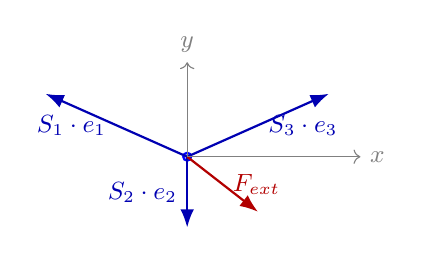
\begin{tikzpicture}[
    node_style/.style={circle, fill=blue!20, draw=blue, thick, inner sep=1pt},
    force_style/.style={-Latex, thick, blue!70!black},
    label_style/.style={font=\small}
]

    % Node at the origin
    \node[node_style] (node_i) at (0,0) {}; 

    % Forces
    \draw[force_style] (node_i.center) -- node[left, label_style] {$S_1 \cdot e_1$} (-1.8, 0.8);
    \draw[force_style] (node_i.center) -- node[left, label_style] {$S_2 \cdot e_2$} (0, -0.9);
    \draw[force_style] (node_i.center) -- node[right, label_style] {$S_3 \cdot e_3$} (1.8, 0.8);

    % External force (optional, but good for context)
    \draw[force_style, red!70!black] (node_i.center) -- node[right, label_style, red!70!black] {$F_{ext}$} (0.9, -0.7);

    % Coordinate system (optional, but good for context)
    \draw[->, gray] (0,0) -- (2.2,0) node[right, label_style] {$x$};
    \draw[->, gray] (0,0) -- (0,1.2) node[above, label_style] {$y$};

\end{tikzpicture}
\end{document}
